\title{Citrine Challenge}
\author{John Goiri}
\date{\today}


\documentclass[12pt, fleqn]{article}
\usepackage{amsmath}
\usepackage{amsfonts}
\usepackage{graphicx}
\usepackage{sidecap}
\usepackage{multicol}
\usepackage[small]{caption}
\usepackage{amsfonts}
\usepackage{breqn}
\usepackage{cancel}
\usepackage{graphicx}

\newcommand{\code}[1]{\texttt{#1}}
\renewcommand{\thesubsection}{\thesection.\alph{subsection}}
\renewcommand{\thesubsubsection}{\thesubsection.\alph{subsubsection}}
\begin{document}
\maketitle

\section{The general idea}
The goal of the challenge is to uniformly sample a subspace within a unit hypercube defined by a series of constraints from the user.
Since the constraints might be non-linear, finding the precise boundaries of the allowed subspace is cumbersome, so I rely on a stochastic approach to navigate my way around.
Starting at the provided feasible point, I sample points nearby, which are more likely to be within the allowed subspace than random points anywhere in the hypercube.
As I find more feasible points, the locations where I'm guessing where the next point is begin to spread.
Once I have sampled enough points, I run them through a ``diffusion'' process, which allows the points to further permeate the subspace for more uniform sampling.

\section{Selecting the probability distribution}
Rather than picking a uniform distribution, I want to sample points that are reasonably close to a feasible point, since blindly sampling for a narrow subspace could take an unreasonable amount of time.
The first step is edge detection, done with the \code{EdgeDetector} class.

Starting with a feasible point, \code{EdgeDetector} will perform a binary search along all Cartesian unit vector directions until it hits the boundary between feasible and not-feasible space.
The distances between the boundaries along positive and negative directions are then used to construct a covariance matrix for a multivariate normal distribution, centered around the feasible point.
Ideally the covariance matrix could be constructed more intelligently to extend as much into the allowed subspace as possible, but I picked the Cartesian directions for simplicity.

Combining an \code{EdgeDetector} and a feasible point, a \code{SourceDistribution} object can be constructed, which uses the multivariate normal distribution to sample points near the feasible point, and returns their coordinates along with their probability density.

\section{Sampling uniformly}
Since the sampled points in the allowed subspace should be uniform, it won't work to just sample from the \code{SourceDistribution} of the initial feasible point, since it will result in clustering around the feasible point.
Instead, the \code{SpaceSampler} class constructs the list of sampled points by creating a new \code{SourceDistribution} for each new point.
As the list grows, there are more candidates that can serve as the center of the new distribution.
Points that had a lower probability of being selected (further from the mean of the distribution they came from) are biased such that they are more likely to be chosen as a feasible point from which to center the new \code{SourceDistribution}.
This new \code{SourceDistribution} will yield the next point in the list of feasible points.

The chances of being a candidate to center a \code{SourceDistribution} are proportional to the inverse of the probability density.
In this manner, the selection of new points spreads away instead of clustering together.

\begin{figure}[h]
    \begin{center}
        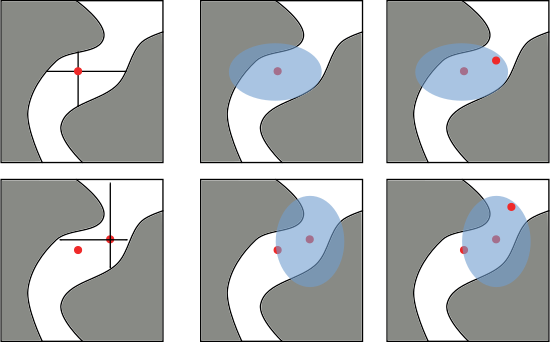
\includegraphics[width=\linewidth]{./detection_sampling.pdf}
        \caption{On the left, using edge detection to find the boundaries of the subspace of a selected feasible point.
        In the center, the lengths of the edge distances are used to create a normal distribution centered about the feasible point.
    On the right, a new feasible point is selected using the probability distribution of the previous step.
The process is repeated until enough points are sampled.}
    \end{center}
\end{figure}

\section{Adding additional uniformity}
Depending on the topology of the allowed subspace, situations may arise where penetrating narrow regions becomes difficult.
If the number of samples are constructed too quickly, then the sampling will only be uniform locally, but may leave sections of the allowed subspace unexplored.
In order to remedy this, I added a ``diffusion'' step that lasts as long as the time limit specified in the prompt (5 minutes).
During this phase, a similar process is applied as during the initial enumeration of feasible points.
This time, when a new point is found, it replaces an existing point so that the list stays the same length.
The chances of being eliminated from the list are proportional to the point's probability density.

Both the initial sampling and diffusion are encapsulated by the \code{SpaceSampler} class.
\end{document}
